%%
%% Template conclusion.tex
%%

\chapter{User Preferences}
\label{cha:ivg}

demographics gender and age are predictive

In this section we will discuss the effects of applying different types of \emph{User Preferences} as the feature vector and 
their predictive tendencies within our data set.

\section{Demographics}
\label{sec:demo}

The \emph{Demographics} data we are interested in includes:
\begin{itemize}
\item \textbf{Age}
\item \textbf{Birthday}
\item \textbf{Locale}
\end{itemize}

Below we will give a basic analysis of the \emph{Demographics} data when extracted from our data set.

Gender breakdown:
% select count(*), lu.gender from linkrUser lu where lu.uid in (SELECT distinct uid FROM trackRecommendedLinks) group by gender;

\begin{table}[!htbp]
\centering
	\begin{tabular}{|c|c|c|} % cols: (left, center, right)
		\hline
		\textbf{Male} & \textbf{Female} & \textbf{Undisclosed}  \\ \hline
		85 & 33 & 1 \\ \hline
	\end{tabular}
	\caption{Gender breakdown for users.}
	\label{tab:revpol}
\end{table}

Despite this clear male bias \cite{jugand} found that in a social setting, there are no strong gender homophily tendencies. Hence the male 
skew should not negatively affect our results. Additionally \cite{backstrom2011center} have shown that different genders have differing 
tendencies to disperse interactions across genders, implying our male skew should be unimportant. Hence gender information will be used in 
the \emph{Demographics} feature vector.

\clearpage

Birthday breakdown:

% select count(*), right(lu.birthday,4) from linkrUser lu where lu.uid in (SELECT distinct uid FROM trackRecommendedLinks) group by right(lu.birthday,4);
\begin{table}[!htbp]
\centering
	\begin{tabular}{|l|c|} % cols: (left, center, right)
		\hline
		\textbf{Year} & \textbf{Frequency}  \\ \hline
		Undisclosed & 1 \\ \hline
		1901-1905 & 1 \\ \hline
		1906-1910 & 0 \\ \hline
		1911-1915 & 1 \\ \hline
		1916-1920 & 0 \\ \hline
		1921-1925 & 0 \\ \hline
		1926-1930 & 0 \\ \hline
		1931-1935 & 0 \\ \hline
		1936-1940 & 1 \\ \hline
		1941-1945 & 0 \\ \hline
		1946-1950 & 0 \\ \hline
		1951-1955 & 0 \\ \hline
		1956-1960 & 2 \\ \hline
		1961-1965 & 1 \\ \hline
		1966-1970 & 4 \\ \hline
		1971-1975 & 10 \\ \hline
		1976-1980 & 12 \\ \hline
		1981-1985 & 25 \\ \hline
		1986-1990 & 34 \\ \hline
		1991-1995 & 25 \\ \hline
		1996-2000 & 2 \\ \hline
	\end{tabular}
	\caption{Birthday breakdown}
	\label{tab:revpol}
\end{table}

Birthdays are grouped in a distinct range, most users in this data set are grouped in the age ranges of ~$\{18 - 30\}$. \cite{jugand} have 
found that there is a strong effect of age on friendship preferences. Hence birthday information will be used in this feature vector.

\clearpage

%select ll.name, count(*) from linkrUser lu join linkrLocation ll on lu.uid in (SELECT distinct uid FROM trackRecommendedLinks) and lu.location_id = ll.id group by lu.location_id;
Location breakdown:

\begin{table}[!htbp]
\centering
	\begin{tabular}{|l|c|} % cols: (left, center, right)
		\hline
		\textbf{Location} & \textbf{Frequency}  \\ \hline
		Undisclosed & 33 \\ \hline
		Ahmedabad, India & 1 \\ \hline
		Bangi, Malaysia & 1 \\ \hline
		Bathurst, New South Wales & 1 \\ \hline
		Bellevue, Washington & 1 \\ \hline
		Braddon, Australian Capital Territory, Australia & 1 \\ \hline
		Brisbane, Queensland, Australia & 2 \\ \hline
		Canberra, Australian Capital Territory & 56 \\ \hline
		Culver City, California & 1 \\ \hline
		Frederick, Maryland & 3 \\ \hline
		Geelong, Victoria & 1 \\ \hline
	\end{tabular}
	\caption{Location breakdown}
	\label{tab:revpol}
\end{table}

Given the fact that most users are either situated in the ACT (location of the app development and deployment) or are undisclosed, 
location information will not be used for this feature vector.

For \emph{Demographics} the $I$ of our feature vector $X$ is defined by the following conditions:
\begin{itemize}
\item Whether the user is male.
\item Whether the user is female.
\item Whether the user and any user in the alters set share the same gender.
\item Whether the user and any user in the alters are of a different gender.
\item Whether the user and any user in the alters set share the same birth range.
\end{itemize}




Denote the set of 
$G \in \{m,f\}$

$u = male$
$u = female$
$u = male \land $

$u = male \land \exists male \in \{alters\}$

The alters of $I$ can then be defined as the set of users who have liked the current item $M$.
Each component of $I$ is set to $1$ if any of the alters have meet the conditions described above, in comparison (where required) 
with the user $n$, otherwise it is set to $0$.

\clearpage

Applying this feature vector to our classifiers we obtain:

\begin{figure}[h]
	\begin{center}
		\includegraphics[scale=0.75]{results/demographics/bar_demographics.pdf}
		\caption{Accuracy results using the \emph{Demographics} feature vector.}
	\end{center}
\end{figure}

The \emph{Demographics} feature vector shows our first positive results, this feature vector almost performs as well as our 
SMB baseline for the case of $k = 0$.

\clearpage
	
Comparing \emph{Demographics} against our exposure curve we obtain:
	
\begin{figure}[h]
	\begin{center}
		\includegraphics[scale=0.75]{results/demographics/line_demographics.pdf}
		\caption{Accuracy results for an exposure curve using the \emph{Demographics} feature vector. Note in this case Constant = NB and LR = SVM.}
	\end{center}
\end{figure}

The exposure curve for \emph{Demographics} shows a sizable improvement over our baselines as our $k$ increases. This demonstrates that as the
number of friends who like an item increases, the probability that a user will like that item also increases. This positive corelation between
number of likes and user likes increases with each $k$.

\section{Traits}
\label{sec:traits}

Facebook facilitates a wide variety of user chosen preferences which we have defined as \emph{Traits}. 
These \emph{Traits} allow users to define under a specific area of their profile different areas or activities they are interested in 
or associate with.

User \emph{Traits} we will investigate include:
\begin{itemize}
\item Activities
\item Books
\item Athletes
\item Teams
\item Inspirational People
\item Interests
\item Movies
\item Music
\item Sports
\item Television
\end{itemize}

Below we display graphs for the different \emph{Traits} sets extracted from our data set. Followed by a subsequent analysis.
Each table shows only the frequency of app users for each of the \emph{Traits}.


The \emph{Traits} graphed above can be broken down into three distinct sets based on their locality within the app user base.

\begin{itemize}
\item \textbf{High Locality}: \emph{Music}, \emph{Movies}, \emph{Television} - Showing our app users appear to share similar \emph{Traits} in a media 
setting.
\item \textbf{Medium Locality}: \emph{Activities}, \emph{Books}, \emph{Interests}, \emph{Sports} - Showing our app users share some degree of similar preferences 
across these \emph{Traits}.
\item \textbf{Low Locality}: \emph{Inspirational People}, \emph{Athletes}, \emph{Teams} - Showing our app users do not share many similar preferences  
across these \emph{Traits}.
\end{itemize}

For each \emph{Traits} group the $I$ of our feature vector $X$ is defined by the following conditions:
\begin{itemize}
\item $I \in \{Activities, Books, Athletes, Teams, Inspirational People, Interests, Music, 
\\ Movies, Sports, Television\}$.
\end{itemize}

The alters of $I$ can then be defined as the set of users who have liked the current item $M$.
Each component of $I$ is set to $1$ if any of the alters have meet the conditions described above for each $t$, in comparison 
with the user $n$, otherwise it is set to $0$.

\clearpage

Applying this feature vector to our classifiers we obtain:

\begin{figure}[h]
	\begin{center}
		\includegraphics[scale=0.75]{results/traits/bar_traits.pdf}
		\caption{Accuracy results using the \emph{Traits} feature vector.}
	\end{center}
\end{figure}

The \emph{Traits} feature vector shows our first improvement over our SMB baseline in the LR and SVM case for $k=0$ demonstrating that 
\emph{Traits} are more predictive then user likes for any previously applied method.

\clearpage

Comparing \emph{Traits} against our exposure curve we obtain:

\begin{figure}[h]
	\begin{center}
		\includegraphics[scale=0.75]{results/traits/line_traits.pdf}
		\caption{Accuracy results for an exposure curve using the \emph{Traits} feature vector.}
	\end{center}
\end{figure}

This trend continues across the exposure curve where each successive increase of $k$ causes the performance of our classifiers to increase.

\clearpage

By extracting the model weights from the case where $k=0$ we can see which \emph{Traits} contain the most predictive qualities:

\begin{table}[h]
\begin{minipage}[b]{1.0\textwidth}
\centering
  \begin{tabular}{|l|l|l|l|} % cols: (left, center, right)
  \hline
  		\textbf{Trait} & \textbf{Weight} & \textbf{Frequency} \\ \hline
		Activities & -5.927 $\pm$ 0.001 & 281 \\ \hline
		Television & -5.210 $\pm$ 0.0 & 1,029 \\ \hline
		Music & -3.409 $\pm$ 0.001 & 629 \\ \hline
		Movies & -2.668 $\pm$ 0.001 & 454 \\ \hline
		Interests & -1.921 $\pm$ 0.001 & 64 \\ \hline
		Sports & -1.820 $\pm$ 0.001 & 27 \\ \hline		
		Books & -1.769 $\pm$ 0.0 & 163 \\ \hline		
  \end{tabular}
  \caption{\emph{Logistic Regression} feature weights extracted for the case where $k=0$. The \emph{Trait} column shows which \emph{Trait}
  is being displayed. The \emph{Weight} column shows the weighting given for this \emph{Trait}. The \emph{Yes'} column displays the number of times 
  this feature vector was set to $1$ for a user and the \emph{Distinct} column displays the number of unique times the feature vector 
  was set to $1$.}
\end{minipage}
\end{table}

This shows us that \emph{Traits} which exhibit a medium to high degree of locality have a larger influence during classification. 
\cite{brandtzag2011facebook} found that virtual interactions help reveal common interests, while real world interactions helps 
to support friendships. These common interests investigated above are clearly predictive of user likes.

\clearpage

\section{Groups}
\label{sec:groups}

Facebook facilitates users to join \emph{Groups} for a large and varied set of different types ranging from 
local sports teams and political preferences to computer games.

\clearpage

The most popular groups for our app users are shown below:

% select count(*),id,name from linkrGroups where uid in (select distinct uid from trackRecommendedLinks) group by id having count(*) > " + minSize + " and count(*) < " + maxSize + " order by count(*) desc;

\begin{table}[!htbp]
\centering
	\begin{tabular}{|l|l|} % cols: (left, center, right)
		\hline
		\textbf{\small{Group Name}} & \textbf{\small{Frequency}}  \\ \hline
		27 & \small{ANU StalkerSpace} \\ \hline
		20 & \small{Facebook Developers} \\ \hline
		15 & \small{ANU CSSA} \\ \hline
		14 & \small{CSSA} \\ \hline
		13 & \small{Australian National University} \\ \hline
		11 & \small{ANU - ML and AI Stanford Course} \\ \hline
		10 & \small{iDiscount ANU} \\ \hline
		10 & \small{Our Hero: Clem Baker-Finch} \\ \hline
		9 & \small{Students In Canberra} \\ \hline
		7 & \small{I grew up in Australia in the 90s} \\ \hline
		7 & \small{Grow up Australia - R18+ Rating for Computer Games} \\ \hline
		7 & \small{ANU Engineering Students' Association (ANUESA) 2010} \\ \hline
		7 & \small{ANU Postgraduate and Research Student Association (PARSA)} \\ \hline
		6 & \small{No, I Don't Care If I Die At 12AM, I Refuse To Pass On Your Chain Letter.} \\ \hline
		6 & \small{No Australian Internet Censorship} \\ \hline
		6 & \small{The Chaser Appreciation Society} \\ \hline
		6 & \small{Feed a Child with a Click} \\ \hline
		6 & \small{ANU Mathematics Society} \\ \hline
		6 & \small{ANU International Student Services, CRICOS Provider Number 00120C} \\ \hline
		6 & \small{2011 New \& Returning Burton \& Garran Hall} \\ \hline
		5 & \small{If You Can't Differentiate Between "Your" and "You're" You Deserve To Die} \\ \hline
		5 & \small{Keep the ANU Supermarket!!!} \\ \hline
		5 & \small{If 1m people join, girlfriend will let me turn our house into a pirate ship} \\ \hline
		5 & \small{The Great Australian Internet Blackout} \\ \hline
		5 & \small{When I was your age, Pluto was a planet.} \\ \hline
	\end{tabular}
	\caption{App users popular \emph{Groups} breakdown.}
	\label{tab:revpol}
\end{table}

\clearpage

In comparison with \emph{Traits}, \emph{Groups} show a higher locality among the most popular groups.

Given the quantity of groups on Facebook, we need to find some optimal test size $j$ for our data set. 
Given memory and time constraints we tested within a range of $\{100-1000\}$ with an incremental step size of $100$ for each test.

\clearpage

The results for these tests are shown below:

\begin{figure}[h]
	\begin{center}
		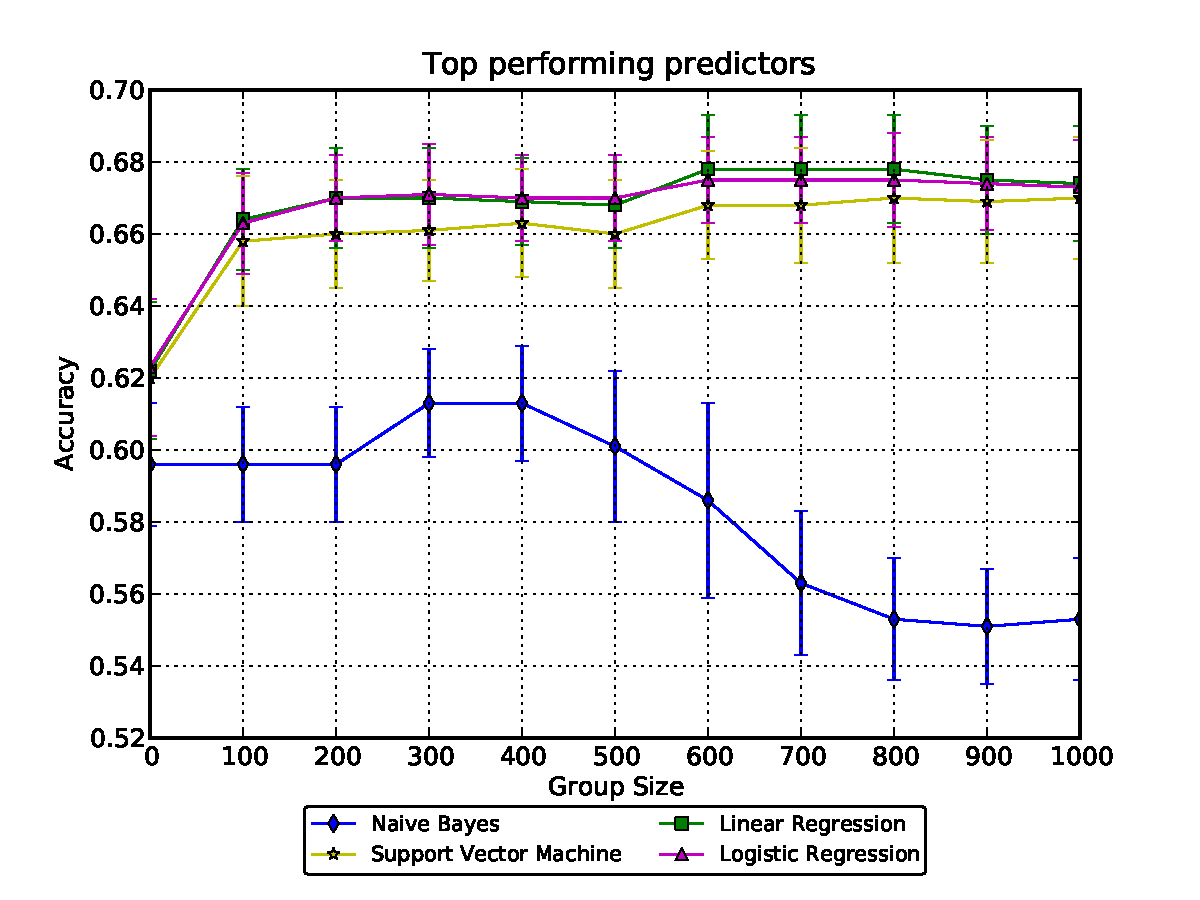
\includegraphics[scale=0.75]{results/groups/top_groups.pdf}
		\caption{Accuracy results for different \emph{Groups} sizes}
	\end{center}
\end{figure}

More gruops help. Localitly.

The most predictive \emph{Group} sizes $j$ for each of our classifiers are:
\begin{itemize}
\item \textbf{Naive Bayes}: 300
\item \textbf{Logistic Regression}: 900
\item \textbf{Support Vector Machine}: 800
\end{itemize}

LR and SVM show a gradual increase as this group size increases, alluding to the possibility of an even higher group size being optimal.

For \emph{Groups} the $I$ of our feature vector $X$ contains an element $i$ for each of the top $j$ groups sizes defined above.

The alters of $I$ can then be defined as all users who have liked the current item $M$.
Each component of $I$ is set to $1$ if any of the alters are a member of the current group $j$ where $i = j$ along with the 
current user $n$, otherwise it is set to $0$.

\clearpage

Using the most predictive \emph{Group} sizes $j$ for each of our classifiers as defined above and comparing to our baselines we obtain:

\begin{figure}[h]
	\begin{center}
		\includegraphics[scale=0.75]{results/groups/bar_groups.pdf}
		\caption{Accuracy results using the \emph{Groups} feature vector.}
	\end{center}
\end{figure}

Both LR and SVM show an improvement over our SMB baseline for the case of $k = 0$ demonstrating that \emph{Groups} are more predictive then 
previous methods.

\clearpage

Applying the \emph{Groups} feature vector across our exposure curve, we obtain:

\begin{figure}[h]
	\begin{center}
		\includegraphics[scale=0.75]{results/groups/line_groups.pdf}
		\caption{Accuracy results for an exposure curve using the \emph{Groups} feature vector.}
	\end{center}
\end{figure}

This trend continues across the exposure curve where each successive increase of $k$ causes the performance of our LR and SVM classifiers to 
increase.

\clearpage

By extracting the model weights from the case where $k=0$ we can see which \emph{Groups} contain the most predictive qualities:

\begin{table}[h]
\begin{minipage}[b]{1.0\textwidth}
\centering
  \begin{tabular}{|l|l|l|l|l|} % cols: (left, center, right)
  \hline
  \textbf{Name} & \textbf{Size} & \textbf{Weight} & \textbf{Frequency} \\ \hline
ANU StalkerSpace & 1292 & -7.236 $\pm$ 0 & 453 \\ \hline
Facebook Developers & 487 & -3.442 $\pm$ 0 & 177 \\ \hline
ANU CSSA & 38 & -2.742 $\pm$ 0 & 191 \\ \hline
Australian National University & 619 & -2.565 $\pm$ 0 & 70 \\ \hline
Overheard at the Ateneo de Manila University & 253 & -2.462 $\pm$ 0 & 26 \\ \hline
iDiscount ANU & 338 & -2.203 $\pm$ 0 & 88 \\ \hline
PETITION FOR FACEBOOK TO INSTALL A DISLIKE BUTTON & 683 & -2.018 $\pm$ 0 & 92 \\ \hline
I grew up in Australia in the 90s & 731 & -1.991 $\pm$ 0 & 75 \\ \hline
Grow up Australia - R18+ Rating for Computer Games & 222 & -1.951 $\pm$ 0 & 102 \\ \hline
Heavy Metal - CANBERRA METAL & 30 & -1.694 $\pm$ 0 & 42 \\ \hline
  \end{tabular}
  \caption{\emph{Logistic Regression} feature weights extracted for the case where $k=0$. The \emph{Name} column displays the name of the feature vector.
                        \emph{Size} represents the size of the \emph{Page} or \emph{Group}.
                        \emph{Weight} represents the weight this feature vector received.  
                        \emph{Yes'} column displays the number of times this feature vector was set to $1$ for a user.
                        \emph{Distinct} column displays the number of unique times the feature vector was set to $1$.}
\end{minipage}
\end{table}

\emph{Groups} of a relatively small size, but a relatively high concentration of app users appear to be most predictive of user 
preferences.

\section{Pages}
\label{sec:pages}

Facebook facilitates users to like \emph{Pages} for 'things' they like across a large and varied set of different areas ranging from 
web browsers and TV shows to schools.

\clearpage

The most popular \emph{Pages} liked by our app users are shown below:

\begin{table}[!htbp]
\centering
	\begin{tabular}{|l|l|} % cols: (left, center, right)
		\hline
		\textbf{\small{Page Name}} & \textbf{\small{Frequency}}  \\ \hline
		33 & \small{ANU Computer Science Students' Association (ANU CSSA) 2011} \\ \hline
		32 & \small{The Australian National University} \\ \hline
		31 & \small{ANU Stalkerspace} \\ \hline
		21 & \small{Humans vs Zombies @ ANU} \\ \hline
		20 & \small{The Big Bang Theory} \\ \hline
		19 & \small{Australian National University} \\ \hline
		19 & \small{How I Met Your Mother} \\ \hline
		18 & \small{ANU LinkR} \\ \hline
		18 & \small{ANU ducks} \\ \hline
		17 & \small{Australian National University Students' Association} \\ \hline
		16 & \small{Google} \\ \hline
		15 & \small{Google Chrome} \\ \hline
		15 & \small{ANU XSA} \\ \hline
		15 & \small{Facebook} \\ \hline
		14 & \small{YouTube} \\ \hline
		14 & \small{The Simpsons} \\ \hline
		13 & \small{Portal} \\ \hline
		13 & \small{Top Gear} \\ \hline
		13 & \small{Music} \\ \hline
		13 & \small{ANU Memes} \\ \hline
		12 & \small{Futurama} \\ \hline
		12 & \small{Scrubs} \\ \hline
		12 & \small{ANU O-Week 2012: Escape to the East} \\ \hline
		12 & \small{The Stig} \\ \hline
		11 & \small{Black Books} \\ \hline
	\end{tabular}
	\caption{App users \emph{Pages} breakdown.}
	\label{tab:revpol}
\end{table}

In comparison with \emph{Traits} and \emph{Groups}, \emph{Pages} show a higher locality across the most popular pages for app users.

Given the quantity of \emph{Pages} on Facebook, we need to find some optimal test size $j$ for our data set. Given memory and time constraints we tested 
within a range of $\{100-1000\}$ with an incremental step size of $100$ for each test.

\clearpage

The results for these tests are shown below:

\begin{figure}[h]
	\begin{center}
		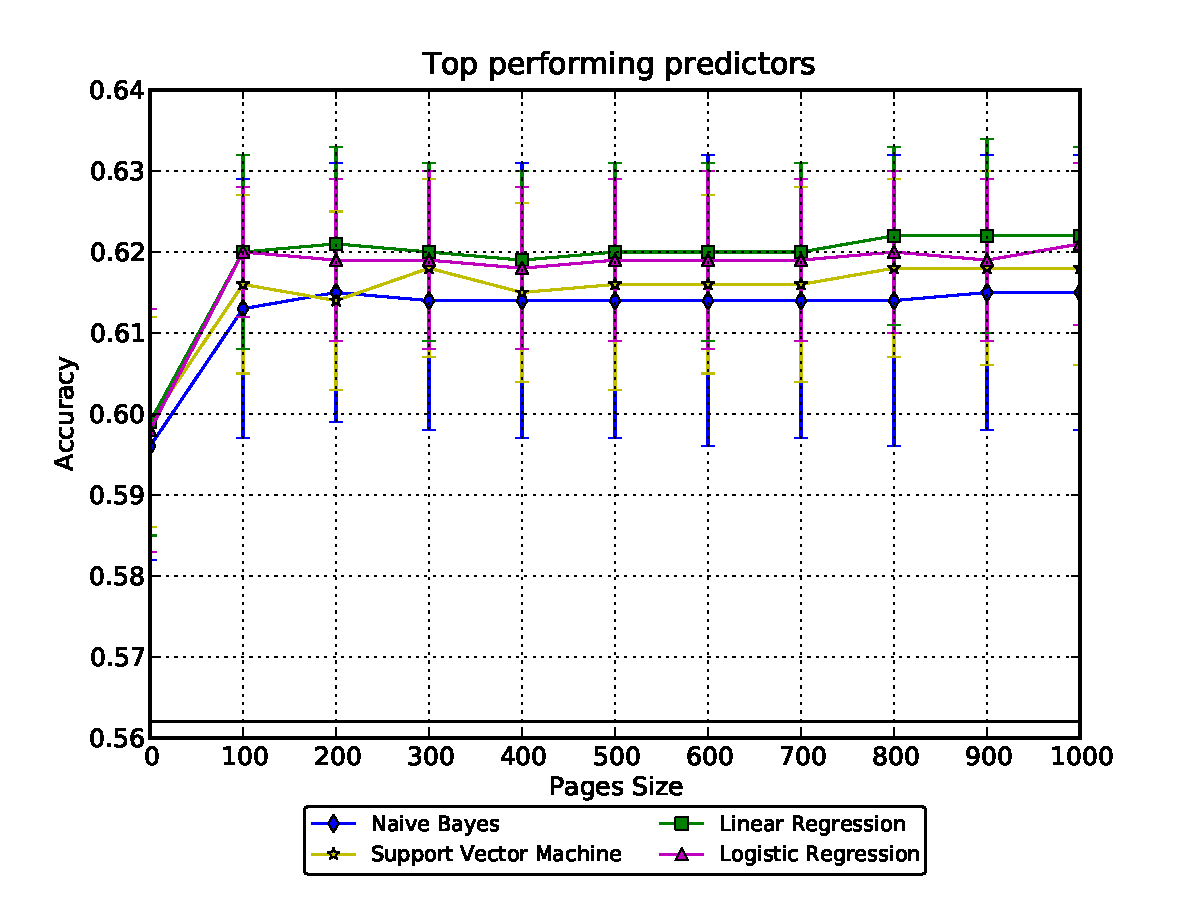
\includegraphics[scale=0.75]{results/pages/top_pages.pdf}
		\caption{Accuracy results for different \emph{Pages} sizes.}
	\end{center}
\end{figure}

The most predictive \emph{Page} sizes $j$ for each of our classifiers are:
\begin{itemize}
\item Naive Bayes: 500
\item Logistic Regression: 900
\item Support Vector Machine: 800
\end{itemize}

LR and SVM show a gradual increase as this group size increases, alluding to the possibility of an even higher page size being optimal.

For \emph{Pages} the $I$ of our feature vector $X$ contains an element $i$ for each of the top $j$ page sizes defined above.

The alters of $I$ can then be defined as all users who have liked the current item $M$.
Each component of $I$ is set to $1$ if any of the alters are a member of the current page $j$ where $i = j$ along with the 
current user $n$, otherwise it is set to $0$.

\clearpage

Using the most predictive \emph{Page} sizes $j$ for each of our classifiers as defined above and comparing to our baselines we obtain:

\begin{figure}[h]
	\begin{center}
		\includegraphics[scale=0.75]{results/pages/bar_pages.pdf}
		\caption{Accuracy results using the \emph{Pages} feature vector.}
	\end{center}
\end{figure}

Improvement over SMB, but not groups. Perhaps because more local.

Both NB, LR and SVM show an improvement over our SMB baseline for the case of $k = 0$ demonstrating that \emph{Pages} are also 
more predictive then previous methods.

\clearpage

Applying the \emph{Pages} feature vector across our exposure curve, we obtain:

\begin{figure}[h]
	\begin{center}
		\includegraphics[scale=0.75]{results/pages/line_pages.pdf}
		\caption{Accuracy results for an exposure curve using the \emph{Pages} feature vector.}
	\end{center}
\end{figure}

This trend continues across the exposure curve where each successive increase of $k$ causes the performance of our LR and SVM classifiers to 
increase.

\clearpage

By extracting the model weights from the case where $k=0$ we can see which \emph{Pages} contain the most predictive qualities:
\begin{table}[h]
\begin{minipage}[b]{1.0\textwidth}
\centering
  \begin{tabular}{|l|l|l|l|l|} % cols: (left, center, right)
  \hline
  \textbf{Name} & \textbf{Size} & \textbf{Weight} & \textbf{Frequency} \\ \hline
Sorry mate i can't, i've got Quidditch  & 254 & -1.799 $\pm$ 0 & 18 \\ \hline
Avatar: The Last Airbender  & 324 & -1.514 $\pm$ 0.001 & 13 \\ \hline
National Geographic  & 662 & -1.437 $\pm$ 0.001 & 18 \\ \hline
The Simpsons  & 1552 & -1.414 $\pm$ 0 & 170 \\ \hline
Sushi  & 387 & -1.33 $\pm$ 0.001 & 9 \\ \hline
House  & 1746 & -1.291 $\pm$ 0 & 66 \\ \hline
Seinfeld  & 609 & -1.249 $\pm$ 0 & 15 \\ \hline
Starbucks  & 1548 & -1.249 $\pm$ 0 & 7 \\ \hline
American Dad  & 540 & -1.215 $\pm$ 0.001 & 18 \\ \hline
friends don't let friends vote for Tony Abbott  & 551 & -1.206 $\pm$ 0.001 & 19 \\ \hline
  \end{tabular}
  \caption{\emph{Logistic Regression} negative feature weights extracted for the case where $k=0$. The \emph{Name} column displays the name of the feature vector.
                        \emph{Size} represents the size of the \emph{Page} or \emph{Group}.
                        \emph{Weight} represents the weight this feature vector received.  
                        \emph{Yes'} column displays the number of times this feature vector was set to $1$ for a user.
                        \emph{Distinct} column displays the number of unique times the feature vector was set to $1$.}
\end{minipage}
\end{table}

\begin{table}[h]
\begin{minipage}[b]{1.0\textwidth}
\centering
  \begin{tabular}{|l|l|l|l|l|} % cols: (left, center, right)
  \hline
  \textbf{Name} & \textbf{Size} & \textbf{Weight} & \textbf{Frequency} \\ \hline

CatDog  & 259 & 1.815 $\pm$ 0.001 & 12 \\ \hline
Worst. Idea. Ever. [pause] Let's do it.  & 227 & 1.737 $\pm$ 0 & 21 \\ \hline
Grug  & 279 & 1.698 $\pm$ 0 & 9 \\ \hline
Kings Of Leon  & 840 & 1.607 $\pm$ 0.001 & 14 \\ \hline
Planking Australia  & 166 & 1.598 $\pm$ 0.001 & 4 \\ \hline
Dr. House  & 964 & 1.588 $\pm$ 0 & 28 \\ \hline
Suit Up  & 466 & 1.389 $\pm$ 0.001 & 17 \\ \hline
Don't you hate it when Gandalf marks your exam and [..]  & 110 & 1.372 $\pm$ 0.001 & 19 \\ \hline
Paramore  & 1004 & 1.343 $\pm$ 0.001 & 31 \\ \hline
Tintin  & 250 & 1.339 $\pm$ 0.001 & 11 \\ \hline
  \end{tabular}
  \caption{\emph{Logistic Regression} feature weights extracted for the case where $k=0$. The \emph{Name} column displays the name of the feature vector.
                        \emph{Size} represents the size of the \emph{Page} or \emph{Group}.
                        \emph{Weight} represents the weight this feature vector received.  
                        \emph{Yes'} column displays the number of times this feature vector was set to $1$ for a user.
                        \emph{Distinct} column displays the number of unique times the feature vector was set to $1$.}
\end{minipage}
\end{table}

The most predictive \emph{Pages} in our data set are ones which contain a larger number of members and a lower concentration of 
app users.

\section{Conclusion}
\label{sec:conc}

Throughout this section we have explored different avenues available for users to demonstrate their personal preferences across a range of 
different mediums.

We have found that \emph{User Preferences} are predictive of user likes, particularly for \emph{Traits}, \emph{Groups} and \emph{Pages}. This 
holds true for the case of $k = 0$ and continues to improve with each successive $k$.

Similarly as with \emph{User Interactions}, our results have shown, that it is enough for some user to have liked an item to allow our classification 
methodology to increase in predictiveness.

pages, groups more local. higher prediction of localised likes (local news, events, etc).
favourites - high frequency 

%%% Local Variables: 
%%% mode: latex
%%% TeX-master: "thesis"
%%% End: 
